\autsection{Guidance and Navigation during EDL}{Maja Tomicic}

The main objectives of the entry, descent and landing (EDL) phase have two aspects, first is lowering down the velocity of the lander to achieve the soft landing, second is performing a pinpoint landing on a selected suitable landing site and avoiding the potential obstacles and hazards during the landing. This section will cover the second aspect theoretically and analytically. 

The requirements for the soft landing depend on the structure of the spacecraft and the payload. Requirements for previous space missions, such as the Mars Science Laboratory was that the spacecraft should touchdown with a horizontal velocity of less than 0.5 m/s and a vertical velocity less than 1 m/s. This order of magnitude is also relevant for this mission. The landing spot has been chosen in advanced based on telescope and ice-penetrating radar images of the surface. The landing module should be able to land in a radius of no more than 100 m from the desired point. 

Because of the distance from Earth to Europa, human remote operation is impossible during the relatively rapid landing and the landing module requires autonomous real-time on-board processing of data acquired by the navigation sensors. During the EDL the sensors on-board must accurately determine attitude, altitude, velocity and location of the spacecraft relative to the chosen landing point. In the following relevant sensors will be presented. 

\subsection{Attitude determination}

The meaning of the word attitude or orientation of a spacecraft refers to the angular departure of the spacecraft from some chosen reference reference. If a reference set of axis as well as spacecraft axis are chosen, the attitude of the spacecraft can be defined. The attitude can be specified using the x-, y- and z- axis as well as the angles roll $\phi$, pitch $\theta$ and yaw $\psi$, which define the rotation about the three axis respectively. There is no universally accepted way of defining attitude, however for a spacecraft in orbit, as will be the case during the EDL, the z-axis is normally the down axis, meaning the local vertical and the x-axis is chosen in the direction of travel \cite{spacecraft}.

Attitude information is fundamental for spacecraft operation and is typically used to point the payload in the right direction or the solar arrays toward the sun. 

There are two main categories of attitude sensors, and they are often used to complement each
other. The first is the reference sensor which gives a definite pose by measuring the direction of an object
such as the Sun or a star. These sensors can go into eclipse or be blinded, which causes periods without information. The other type are inertial sensors, which measure the attitude continuously, but as the name suggest they measure the changes in attitude in an inertial frame. Their errors progressively increase because of random drifts and the inertial sensors therefore need regular calibration from reference sensors \cite{spacecraft}.

\subsubsection{IMU}
The Inertial Measurement Unit (IMU) measures the spacecraft's angular velocity, orientation and acceleration in an inertial frame with accelerometers and gyroscopes. The data from the IMU is used for calculation of the spacecraft current position and attitude from a given initial value. Because of the bias and drift of the accelerometers and gyroscopes the error of the IMU is accumulated over time, which means that the IMU cannot give correct navigation information relative to the surface alone \cite{IMUcamb}.
To correct for the error other navigation sensors, such as star trackers, are required to work in fusion with the IMU. 



\subsubsection{Star reference sensors}
With an accuracy better than 1 arcsec star sensors are the most accurate reference attitude sensors in common use \cite{spacecraft}. A star tracker consists of a CCD camera and a powerful microcomputer. Sophisticated techniques and image analysis software, identify star patterns within the FOV and by comparing them to catalogue patterns, the absolute attitude of the spacecraft can be determined.  Because stars are point sources and the photon flux is low, the sensor needs long exposure periods. This inherently limits the temporal resolution and frequency of measurements, and affects operations during maneuvers such as braking, since vibrations of the spacecraft will affect the image quality. To ensure unique attitude determination and for redundancy, in case one of the sensors get blinded by the sun or other strong sources, two star sensors should be placed in orthogonal directions and combined with an other attitude determination system such as an IMU \cite{alessandro}.

\subsubsection{Other attitude sensors}
Other than the previously mentioned sensors, sensors such as \textit{sun sensors}, \textit{horizon sensors} and \textit{magnetometers} are often used for spacecraft attitude determination. These sensors are not as accurate as star trackers, however they can be made very light and compact as chip systems, using a minimal amount of power. The principle of these sensors will not be elaborated on in this report. 


\subsection{Altitude}
Altitude measurements yield the height of the spacecraft relative to the surface. Precision altitude data have been shown to significantly improve spacecraft control during the soft-landing process because of the accurate height and descent rate measurements. The descent rate is achieved by differentiating successive altitude readings. Not surprisingly, the data are most critical in the final descent phase where the spacecraft is within $\sim$100 meters to a few meters from the surface. Altitude information can also be used to amend the error of the IMU. 


\subsubsection{Radar Altimeter}
A radar altimeter is a system that measures the distance from the system platform to the surface very accurately. It works on the principle of time of flight. It measures the time delay between a transmitted radar pulse and the detection of the reflected pulse. The altitude of the altimeter, $h$, is related to the time delay of the signal $t_d$ by the simple relationship 

\begin{equation}
h=\dfrac{c t_d}{2}
\end{equation}

where c is the velocity of the signal (speed of light)\cite{henningalt}. The transmitted radar pulse will cover an area on the surface called the radar footprint, $X$, this depends on the height of the altimeter, $h$, and the pulse length, $T$, as follows 

\begin{equation}
X=2\sqrt{cTh}
\end{equation}

The radar pulse length is normally in the range of a few nanometers, which would yield a footprint of $\sim$ 20m at $\sim$ 100 m altitude.

A radar altimeter consist of a transmitting and receiving antenna and a signal processor. The antenna size increases with decreasing footprint.

Errors in the radar retrieval of altitude are often due to inaccurate modeling
of surface penetration or the slope-induced error caused by
the large radar footprint \cite{icealti}. The range resolution of a radar altimeter also depends on the accuracy of the processing clock.


\subsubsection{Laser altimeter}

The principle of a laser altimeter also known as laser range finder is the same as for the radar altimeter. It measures the time delay between the transmitted and received echo signal. The error on the achieved data therefore depends on the on-board clock.

A laser altimeter is composed of an emitter, a receiver and signal processor. Figure \ref{alti} shows an example of a compact laser altimeter. 

The footprint of a laser, is significantly smaller than that of a radar pulse. It depends on the beam divergence and the altitude of laser system. This is illustrated in figure \ref{alti}.  Because of the small footprint the slope-induced error in the measurements is not a concern.

\begin{figure}[htb]
\begin{center}
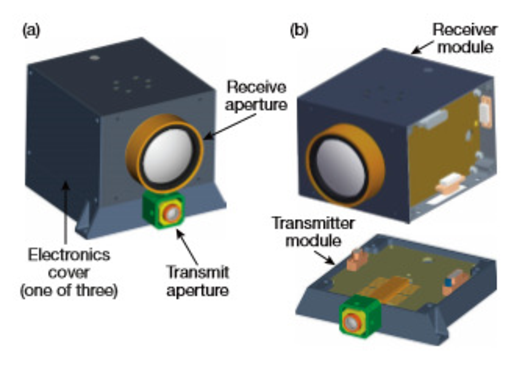
\includegraphics[width=0.45\textwidth]{figures/navtheory/CLA}
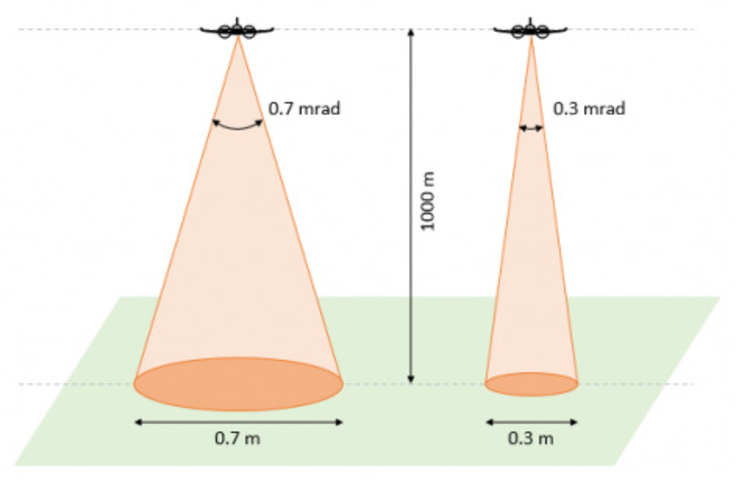
\includegraphics[width=0.45\textwidth]{figures/navtheory/lidarfoot}
\caption{To the right is a sketch of a compact laser altimeter developed by the John Hopkins APL \cite{APLCLA}. To the left is an illustration of how the beam divergence of a laser altimeter changes the laser footprint.\cite{footprint}}
\label{alti}
\end{center}
\end{figure}

One major drawback of laser altimeters compared to radar altimeters is that the laser beam cannot penetrate cloud cover. This will not affect measurements on Europa because of the non existing atmosphere. 

An important property of both the radar and laser altimeter is that they are active sensors and thereby able to exploit more optimal measurement conditions in which surface illumination is controlled by design rather than accommodated by  solar illumination. The downside to this, is that the sensors require more power to run the active illumination compared to a passive instrument. 

There are more sophisticated techniques of laser rangers known as Lidar systems. The principle here is to mix the returned and transmitted signal to achieve an interference signal whose frequency is proportional to the target range. These systems are often in combination with laser velocity measurements systems known as Doppler Lidar and will be elaborated on in the following sections. 



\subsection{Velocity}

Knowing the spacecraft velocity is critical to a soft landing, because it enables the control system to respond to the rapidly changing terrain. Calculating the orbital velocity can be useful to estimate the image optical flow and thereby determine the optimal integration time for surface cameras \cite{alessandro}. The velocity can also be used to amend the error of the IMU.

The velocity of the spacecraft relative to the surface can be broken in two components: vertical and horizontal. As mentioned the vertical component can easily be determined by differentiating successive altimeter readings, the horizontal component requires more processing and more complex measuring techniques of the surroundings. 

\subsubsection{Doppler Radar}
The principle of a doppler radar velocity sensor is that the frequency shift between the transmitted and received echo signal is directly proportional to the velocity of the spacecraft relative to the reflecting surface. This is shown in the following \cite{henningdoppler}. 

The radar transmits a continuous signal given by

\begin{equation}
s_t(t)=\cos (2 \pi f_t t)
\end{equation}


where $f_t$ is the frequency of the transmitted signal. The signal travels
from the radar to the target and back to the radar again, and hence the radar signal
travels a total distance of 2R at the speed of the signal (speed of light), c. The echo signal received by the radar
system is then

\begin{equation}
s_r(t)=a \cos(2 \pi f_t(t-\dfrac{2R(t)}{c}))
\end{equation}

$a$ is a constant that represents the fraction of the energy transmitted from the radar
that is returned to the radar again. The phase of the received signal is seen to be 

\begin{equation}
\phi_r(t)=2 \pi f_t(t-\dfrac{2R(t)}{c})
\end{equation}


The frequency of the received signal is found by differentiating the phase with respect
to time

\begin{equation}
f_r(t)=\dfrac{1}{2 \pi}\dfrac{d\phi}{dt} = f_t - \dfrac{2 f_c}{c}\dfrac{dR(t)}{dt}
\end{equation}

$-\dfrac{dR(t)}{dt}$ is the radial velocity of the spacecraft relative to the surface, and the doppler frequency ($f_d$) is seen to be directly proportional to this velocity:

\begin{equation}
f_d= f_t\dfrac{2 v_r(t)}{c}
\end{equation}

As is evident from the description of the principles, a radar altimeter and doppler velocity sensor can easily be, and are often, combined. 

Many past landing missions, including Surveyor, Apollo, Mars Science Laboratory relied on radar
technology for the altitude and velocity data. These systems are heavy and power consuming and future missions are starting to rely more heavily on doppler lidar systems, which offer major benefits including lower mass, smaller
size, higher precision and data rate. These qualities are particularly critical for deep space mission, when autonomous hazard avoidance is employed or when “pinpoint landing” is required, such as is the case in this mission.


\subsubsection{Doppler Lidar}

The doppler lidar system is based on the principle of lidar where the frequency shift between transmitted and received signals is used to determine the range of the surface. When the lidar platform is not stationary relative to the surface during the  beam round trip time, the signal frequency will be also shifted due to the Doppler effect. Therefore by measuring the frequencies of the laser signals, both the target range and velocity can be
determined. The lidar transmits three separated laser beams in order to determine the three components of the spacecraft velocity, and to accurately measure altitude relative to the surface. 
 

  
\subsubsection{Optical sensor}
An camera directed at the surface can provide enough information to calculate the horizontal velocity parameter. The procedure is based on tracking multiple feature points between successive images and estimating the horizontal velocity from the observed displacement. Attitude information from the IMU and star trackers can be used to correct for difference in rotation and camera pointing between the successive images \cite{alessandro}.

The method is explained in \cite{alessandro} and illustrated in figure \ref{horvel}.

\begin{figure}
\begin{center}
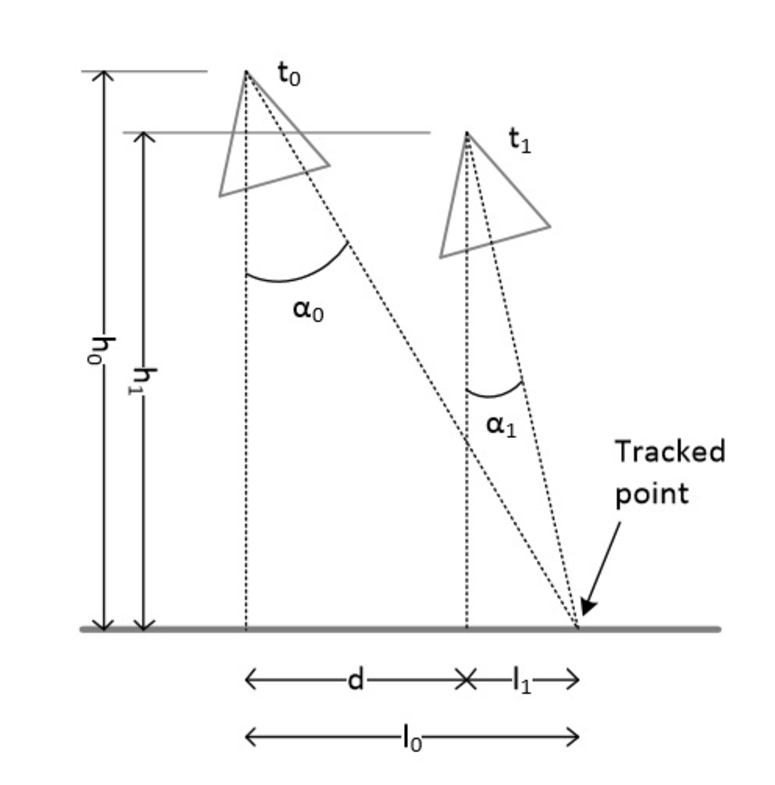
\includegraphics[width=0.5\textwidth]{figures/navtheory/horvel}
\caption{sketch from \cite{alessandro}}
\label{horvel}
\end{center}
\end{figure}


The spacecraft observes a feature point at time $t_0$ and $t_1$ while moving a distance $d$ in the horizontal direction and descending from altitude $h_0$ to $h_1$. According to this geometry, the horizontal velocity can be found as

\begin{equation}
v=\dfrac{d}{t}=\dfrac{l_0-l_1}{t}
\end{equation}

$l_i$ are given by the altitude, the focal length of the camera, the off nadir pitch angle and the rotation corrected point coordinate on the sensor plane, as described in \cite{alessandro}.


The optical camera used for horizontal velocity measurements has to be optimized for its purpose. Because of the rapidly changing terrain due to the high velocity, a camera with a wide FOV is desired to ensure that as large an area as possible is covered and that the feature points are repeated in more frames.


 
\subsection{Optical cameras}

Optical cameras have shown to be very useful for navigation during EDL in spite of the inherent need for ambient light. This is due to their simplicity and compact size. It is vital to design a camera that will provide the necessary ground coverage/FOV and resolution/Ground Sampling Distance. These features depend on the design of the camera, mainly the focal length and sensor characteristics. In the following a breaf analysis of these features will be performed. The analysis can be used to choose fitting camera parameters for the landing module. 

From geometric optics an analysis of FOV and resolution can be made. Figure \ref{cameramatlab} shows the FOV  and GSD at varying altitudes for cameras of different focal lengths, for the $\mu$ASC sensor. The sensor specifications are shown in table \ref{tab:ASC} and are taken from \cite{alessandro}. It is assumed that an object is resolved if it spans two pixels. The matlab code developed for calculating the parameters is attached in the Appendix \ref{app:majamatlab}.

\begin{table}[htb]
\begin{center}
\begin{tabular}{|c|c|c|}
\hline
Optical Bandwidth [nm] & Pixel size [$\mu$m] & Detector size [px]\\
\hline
380-760  & 8.6$\times $8.3 & 752 $\times$ 580 \\
\hline
\end{tabular}

\caption{Specifications for the CCD $\mu$ASC sensor. From \cite{alessandro}.}

\label{tab:ASC}
\end{center}
\end{table}

From figure \ref{cameramatlab} it is seen that the GSD is improved by increasing the focal length of the camera, and might seem as though we can get an arbitrarily good resolution by increasing the focal length and sensor size. However, this is not the case. Eventually a point is reached where the image becomes larger, but does not gain in detail. The best focused spot of light, that a camera with a circular aperture can make, is limited by the diffraction of light. The diffraction pattern formed by a circular aperture consists of a central bright spot, known as an Airy disk, surrounded by a series of bright and dark rings, as shown in figure \ref{airy} \cite{uniphys}.

\begin{figure}[htb]
\begin{center}
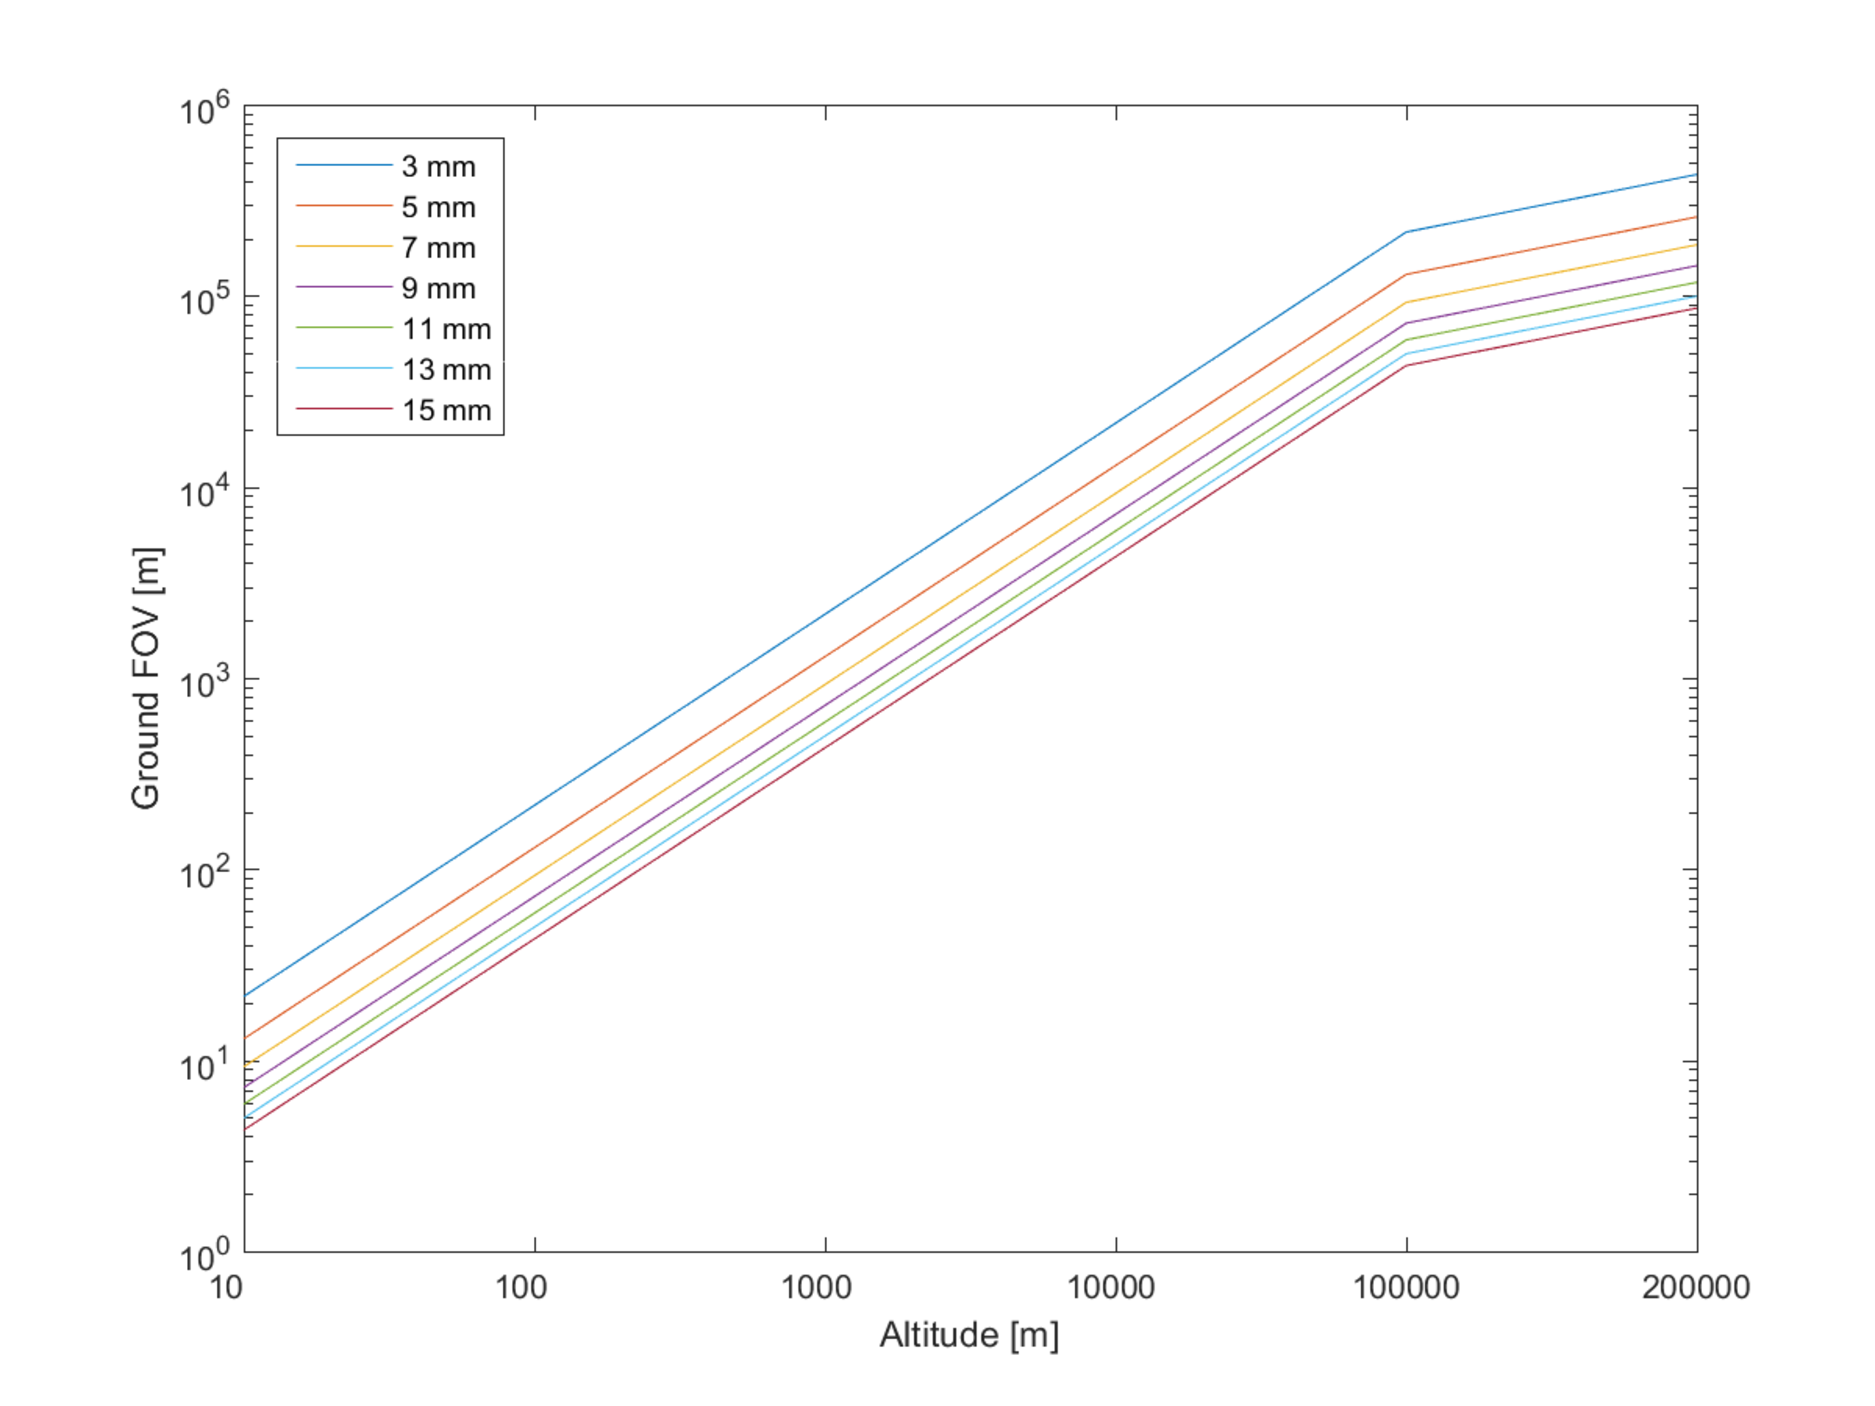
\includegraphics[width=0.7\textwidth]{figures/navtheory/FOV} 
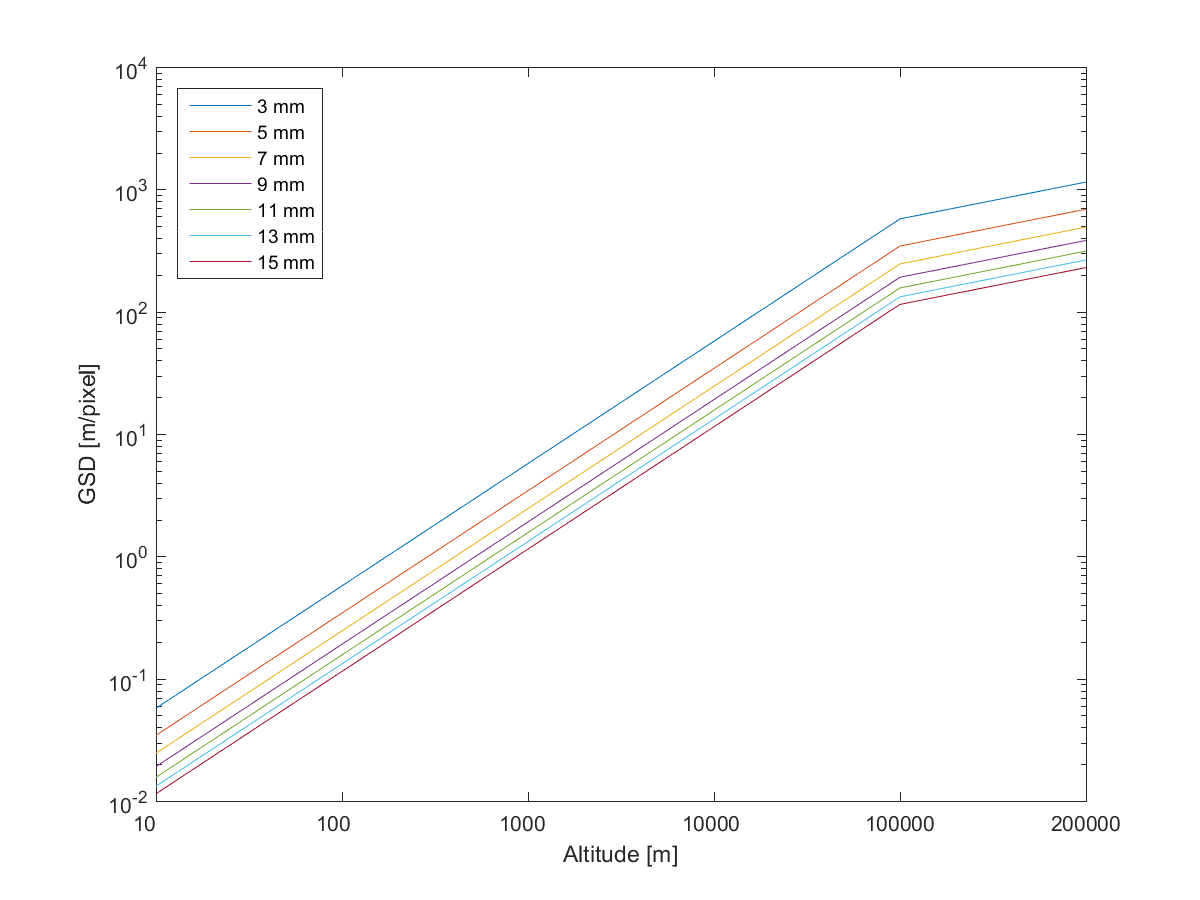
\includegraphics[width=0.7\textwidth]{figures/navtheory/GSD}
\caption{FOV (top) and GSD (bottom) at different altitudes as a function of  camera focal length. }
\label{cameramatlab}
\end{center}
\end{figure}



\begin{figure}[htb]
\begin{center}
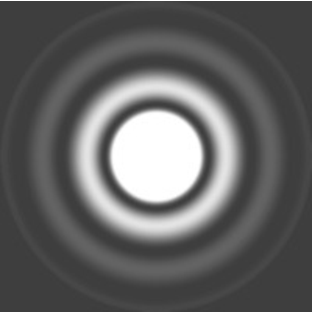
\includegraphics[width=0.5\textwidth]{figures/navtheory/airy}
\caption{Diffraction pattern formed by a circular aperture. The central spot is known as the airy disk and limits the resolution of a optical instrument.}
\label{airy}
\end{center}
\end{figure}

The size of the airy disk depends on the aperture size, $D$, and the wavelength of the focused light, $\lambda$, and can be described in terms of its angular radius $\theta$.

\begin{equation}
\label{eq:diff}
\sin \theta = 1.22 \dfrac{\lambda}{D}
\end{equation}

To determine the resolution of two points from the size of the Airy disk, a widely used criterion is the Rayleigh criterion. It states that two objects are just barely distinguishable if the center of one diffraction pattern coincides with the edge of the Airy disk of the other. Combining the Rayleigh criterion with equation \ref{eq:diff}, the limit of resolution can be determined for an optical system \cite{uniphys}.

A camera system with an aperture of 30 mm and focal length of 7 mm could resolve objects in visible light ($\sim$ 500 nm )at a distance of 100  km of: 

\begin{equation}
\theta\approx \sin \theta=1.22 \dfrac{500 \mathrm{nm}}{30 \mathrm{mm}} = 1.75 \cdot 10^{-5} \mathrm{rad}
\end{equation} 


\begin{equation}
2.0 \cdot 10 ^{-5} \mathrm{rad} \cdot 100 \mathrm{km} = 2.0 \mathrm{m} 
\end{equation}

In the image plane the distance will be

\begin{equation}
2.0 \cdot 10 ^{-5} \mathrm{rad} \cdot 7 \mathrm{mm} = 0.14 \mathrm{\mu m} 
\end{equation}

This is very high resolution, compared most CCD pixel sizes, which are in the $\mu$ m range, and the diffraction limit will not be the limiting factor in this case. 


\subsection{Terrain relative location}


The terrain relative navigation consists of two main parts, terrain mapping and navigation software.
The measurements from the sensors on the spacecraft are input to the terrain mapping algorithm. The estimated position of the spacecraft which is the result of terrain mapping is used as input for the navigation algorithm. The sensors used for terrain mapping is the main focus of the following and the navigation software will not be elaborated on, and could be the subject of future work. 


\subsubsection{Optical camera}

When pre-generated maps of the lunar surface are available, a topographic matching approach, can help land the spacecraft accurately at the desired position. Typical approaches identify crates, cracks and ridges in the observed scene and correlates them to orbital visual images. This requires sophisticated and complex image analysis software but has been done in the past, and seems to be a promising and constantly improving method of relative navigation. The optical CCD camera is a passive measurement sensor, so the power and weight of the equipment can be decreased to a low level. The down side to this type of measurements arise from the nature of the sensor, as they are affected by the illumination conditions. The primary light source is the sun and the visibility therefore depends on the local orientation of the sun. Obviously no features are visible during local night time, but the scene appearance can change dramatically between mornings and evenings when the sun is low on the sky, causing long shadows and midday. These issues can be corrected for in software using inputs from attitude sensors, such as the IMU or a sun sensor, which can determine the relative position of the sun. It has to be evaluated if the lightning conditions change during the landing, or if the lunar rotation period is long enough to make variations in lightning conditions during landing negligible. 


\subsection{Hazard avoidance}

During the last stage of the landing – the terminal descent – at altitudes between approximately one hundred meters and touchdown, many of the finer structures such as rocks, cliffs and cracks on the surface become detectable. During this phase of the landing the guidance and navigation system has to be able to detect and avoid possible hazards as well as choose a suitable landing point. It can no longer rely on catalougue maps, but has to evaluate the terrain in front of it immediately and autonomously. For this, 3D imaging have great advantages over 2D imaging. 



\subsubsection{Stereo camera}
Most low mass low power hazard avoidance sensors, used on e.g. Mars rovers, are stereo camera systems. This approach utilizes triangulation to determine range by matching points in one camera frame to the corresponding point in the other frame. Because the system has no active light source its operation is limited to the daytime. Moreover, stereo correlation algorithms can be sensitive to lighting conditions and contrast of the objects, resulting in ineffective acquiring of 3D data at low contrast or shadowing of the terrain \cite{structuredlight}.
 

\subsubsection{3D flash Lidar}

The principle of the flash Lidar is similar to that of a pin-hole camera. It is composed of a camera, a laser transmitter and a detector plane such as a CCD. After the laser pulse is reflected on the surface, it reaches the detector. The detector array takes an image of the reflected laser signal from a certain area at a time. The image includes intensity and range data of the reflected surface. The intensity data is stored in black-and-white images and the range data is converted to 3D point clouds.
The 3D point cloud enables the Lidar to generate elevation maps of the terrain that indicate hazardous features such as rocks, craters, and slopes. The elevation maps collected during the approach phase of a landing vehicle, at about 1 km above the surface, can be used to determine the most suitable safe landing site. At higher altitudes, the Flash Lidar can generate contour maps of the terrain for matching them with cataloque maps of known surface features, thus also be used for relative navigation prior to the final landing phase.

\subsubsection{Structured light}


A structured light system consists of a light emitter and a camera. The light emitter can be a laser that is passed through a diffraction grating, which splits the laser beam into many individual beams, to generate a pattern (structured illumination). The laser projects the pattern of beams onto the surface in front of the camera. Because each beam is separated from the camera at a known distance and angle, the range can be recovered using triangulation, the same principle used in stereo vision.  \cite{structuredlight}

One obvious challenge when using structured light is the ambient light that will act as a strong source of noise. There are several ways to increase the signal to noise ratio. 

\begin{enumerate}

\item Narrow bandpass filter
\item Pulsed light source and fast camera shutter
\item Background subtraction
\item By increasing the laser power of the laser
\item Choosing a wavelenght where the ambient light is low

\end{enumerate}


Structured light systems can be build very compact,have no moving parts, and consume little power compared to the 3D flash lidar. 


\subsection{Sensors for GNC during EDL}

In the following a range of sensors which have been considered and analyzed are presented. \\

The following IMU's have been considered: 
LN$\-$ 200 FOG Family developed by Northrop Grumman \cite{LN200}, Miniature Internatial Measurement Unit (MIMU) developed by Honeywell \cite{mimu} and the Micro Intertial Reference Unit (MIRU) developed by DTU Space.

As describes previously the IMU cannot stand alone, because it provides attitude information in an inertial frame and the error accumulates over time. By combining it with a star tracker the error is corrected for. 


An integrated system, consisting of a $\mu$ ASC star tracker augmented with a novel inertial reference unit is described in \cite{Bjarno} and developed at DTU Space. With both sensors providing attitude measurements the advantage of the combined system is high accuracy and robustness to cases with long periods of vibrations or camera blinding which are undesirable situations for a attitude determination system consisting of stellar reference sensors alone. Figure \ref{miruasc} shows a MIRU augmented $mu$ASC camera head unit. The MIRU is integrated into the camera head unit of the $\mu$ ASC system, making it 40 g heavier and using 130 mW more power, per camera \cite{mirusheet}. 

\begin{figure}[htb]
\begin{center}
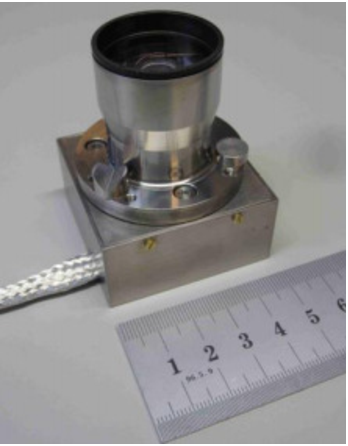
\includegraphics[width=0.5\textwidth]{figures/navtheory/chumiro}
\caption{This image from \cite{mirusheet}, shows the MIRU augmented $\mu$ASC CHU.}
\label{miruasc}
\end{center}
\end{figure}

The $\mu$ASC system consists of two separate units, the Data Processing Unit (DPU) and the Camera Head Unit (CHU). Each DPU, which is fully redundant may drive up to four CHU's and each CHU may be connected to more than one DPU depending on the processing demands of the operation. The $\mu$ASC has the capabilities to support external instruments such as magnetometer and sun sensors if this should be relevant. The CHU's are CCD cameras that can be designed as requested, and it is therefor possible to design one CHU for terrain relative navigation from high altitudes $\sim$100 km and one for low altitudes $\sim$ 10 m. The low altitude CHU can be combined with a laser to form a structured light system and thus be used for hazard avoidance. The optical cameras can be used for velocity information as describes in previous sections and in \cite{alessandro}. And by correlating them with cataloque images of the surface the absolute position can also be determined. 

\begin{sidewaystable}[H]
\begin{flushleft}

\begin{tabular}{|c|c|c|c|c|c|c|c|c|}
\hline 
Instrument & Mass [g] & Power [W] &Attitude & Altitude & V. velocity & H. velocity & Terrain relative & Hazard detection\\ 
\hline
LN$\-$ 200 (IMU) & 750 & 12 & Yes & Inertial & Inertial & Inertial & No & No\\
\hline
MIMU (IMU) & $>$4700 & 22 & Yes& Inertial & Inertial & Inertial & No & No\\
\hline

MIRU (IMU)& 40 & 0.130 & Yes& Inertial & Inertial & Inertial & No & No\\
\hline
$\mu$ASC (Optical)  & 1000XX & XX& Yes & (Yes) & (Yes) & (Yes) & Yes & (Yes)\\
\hline
SF02 (laser ranger) & 69  & 6m & No & Yes  & Yes & No & No & No\\
\hline
SILAT (Optical + Lidar) & 5000  & 12 & No & Yes & Yes & Yes & Yes & Yes \\
\hline
MRA Type 1 (Radar alt.) & 600 & 7& No & Yes  & Yes & No & No & No \\
\hline
APL CLA (Lidar) & 1000 & 7 & No & Yes & Yes & Yes & No& No \\
\hline

 

\end{tabular}
\caption{Score table of instruments that were considered during the process of this project. The parenthesis suggest that the instrument can provide the measurements indirectly or in combination with other instruments. }
\label{tab:sensors}
\end{flushleft}
\end{sidewaystable}


For altitude measurements a range of Laser and Radar systems have been considered. Their specifications are listed in table \ref{tab:sensors}. These sensors can perform autonomous operation under any lighting conditions and any landing location.\\

Lightware’s SF02 laser ranger is a lightweight module that provides fast and accurate distance measurements from 0-50 meters, using pulsed-laser time-of-flight measurements \cite{SF02}. \\

The APL compact laser altimeter (CLA) is a suite consisting of a series of laser ranging sensors paired with  Doppler radar sensors. The laser rangers offer extremely precise vertical distance and surface-relative attitude information, whereas the radars provide equal precision with respect to vertical and horizontal velocities. Additionally, a fourth, nadir-facing sensor pair could offer component redundancy as well as distance information to the landing site directly below the spacecraft \cite{APLCLA}. \\


The Stereo Imaging Laser Altimeter (SILAT) combines two optical cameras with a low-power photon-counting laser altimeter. The result is a multifunctional instrument suite designed for high resolution images for terrain relative navigation, stereoscopic images that can be used for hazard avoidance, and high accuracy altimetry. This combination of instruments will also provide velocity measurements \cite{SILAT}. The SILAT is quite heavy weighing $\sim$ 5 kg, and is therefore ruled out for this mission.\\

A radar altimeter such as the miniature radar altimeter MRA type 1 \cite{MRA1}, has been considered. However it is developed for drone applications and is therefore not qualified for space use yet. Also, as mentioned earlier the footprint of a radar altimeter is larger than that of a laser altimeter, why laser altimeters are more useful for landing purposes.  


\subsection{Conclusion}

The main driving forces in the process of choosing the sensors for the GNC system have been to ensure an autonomous soft pin-point landing within a radius of 100 meters of a predetermined landing spot. The sensors should meet these requirements in a somewhat redundant manner while being both weight and power efficient. 

Optical systems provide the information needed for autonomous navigation. Although having to rely on ambient light, they are intrinsically more accurate and less demanding, in terms of power and mass budgets, than the corresponding radar and laser systems. They are easier to operate and more robust because they passively acquire the signal coming from the observed surface rather than actively tracking it. For these reasons the relative navigation system and hazard avoidance system will rely on optical systems, more specifically on the $\mu$ASC system, with appropriately designed CHU's and in combination with other light weight sensors such as the MIRU and a compact laser ranger. The choice of focal lenght for the CHU will be a compromise between FOV and GSD. For high altitudes a focal length of 13 mm would yield a FOV of $\sim$50 km$^2$ and a GSD of $\sim$130 m/px, which is acceptable . For the final descent, the CHU used for hazard avoidance will have a focal length of 7 mm which yields a FOV of $\sim$ 10 m$^2$ and GSD of $\sim$ 2.5 cm at 10 m altitude. 

Since the orientation of the spacecraft will be different during different phases of descent and landing, it may be difficult to accommodate the cameras such that they will have a clear view of the ground during the approach phase (< 100 m altitude), when it needs to perform hazard avoidance functions, as well as early descent phase (at high altitudes), when altimetry and terrain relative navigation functions need to be performed. This is the advantage of having two CHU's dedicated to terrain imaging. One with long focal length for the early descent phase and one with shorter focal length for the final phase. Because the can be placed on different position on the spacecraft.

The altitude of the spacecraft can be obtained through analysis of optical images in combination with attitude measurements for the initial phases of the landing. Since very precise information is necessary for the final stage, a light weight laser altimeter will be placed on the face of the spacecraft pointing downwards during this stage. 

It has to be evaluated whether an extra flight computer is necessary. The two redundant DPU's should theoretically be able to handle all the processing needs of the landing, however most conventional systems carry an extra flight computer for communication, power, altitude, fail safe conditions etc.

 
\subsubsection{Final guidance and navigation control system}
Initially, the navigation system uses one of the CHU's as a surface camera together with a database of known surface
features (craters, cracks and ridges), two CHU's as star trackers and the integrated IMU system $\mu$IRU. The surface camera is designed to optimize the FOV and resolution for this purpose. This ensures direct position and attitude determination in a Europa fixed frame of reference.
As the lander approaches the moon surface fewer features in the surface camera FOV
can be matched to the database. Therefore the relative velocity navigation system is included
which uses the optical flow from unknown surface features to estimate
the lander velocity with respect to the lunar surface. This is then integrated to give the
position. At altitudes of about 100-50 meters from the surface the laser ranger is used to determine a precise height of the spacecraft relative to the surface. This information is used as hazard avoidance as to avoid deep gorges or steep hills. Finally, as the lander gets the intended landing area in sight, it will navigate
relative to a hazard free landing spot using the last CHU as a surface camera, with optimized optics, together with a laser as a structured light system. 

Final instruments are 

-$\mu$ASC system (including four CHU's with build in IMU (MIRU) and two redundant data processing units (total of four DPU's) )
-two of the cameras are used as star trackers and two as surface cameras with different FOV and resolution (one for high altitudes and one for final landing)
-One laser to be combined with one of the cameras to make a structured light hazard avoidance system
-One laser ranger (range approx. 100 m)


\subsection{Power supply on landing module}

The Guidance Navigation and Control system will be powered by a small RTG. The total system requires 

We considered using solar panels with Fresnel lenses to concentrate the relatively low solar flux at Europa ($51 W/m^2$). However the extreme radiation environment is too harsh for the solar cells to survive for longer periods of time. An option would be to deploy the solar cells down into the ice, and only have the Fresnel lenses in the radiation environment. The process of deploying the large amount of solar cells into the ice was rejected due to its complicated nature. 




